\section{Customizing the tables}\label{pers}

\subsection{\texttt{\textcolor{red}{help}}: an option of the main macros}

\subsubsection{\texttt{\textcolor{red}{help}}: option of \addbs{tkzTabInit}}
This option shows the structure of a table. \tkzname{deltacl=1} spreads the points and the labels a little.

\begin{tkzexample}[small]
  \begin{tikzpicture}
   \tkzTabInit[deltacl=1,espcl=8,help]%
   {$x$/1,Sign\\ of $\dfrac{1}{x}$/1.5/1.5,Variations\\ of $\ln$/2}%
   {$0$,$+\infty$}%
   \end{tikzpicture}
\end{tkzexample}


\subsubsection{\texttt{\textcolor{red}{help}}: option of \addbs{tkzTabLine}}
To see the labels better, do not use the option \tkzname{help} with all the macros at the same time.
\begin{tkzexample}[small]
	\begin{tikzpicture}
	 \tkzTabInit[deltacl=1,espcl=8]%
	 {$x$/1,Sign\\ of $\dfrac{1}{x}$/1.5/1.5,Variations\\ of $\ln$/2}%
	 {$0$,$+\infty$}%
	 \tkzTabLine[help]{,,}%
  \tkzTabVar{D-/ $-\infty$,  +/$+\infty$}
	 \end{tikzpicture}
\end{tkzexample}

\subsubsection{\texttt{\textcolor{red}{help}}: option of \addbs{tkzTabVar}}
This option shows the nodes used to draw the arrows of variation. To avoid too many labels, only the nodes that are used are named. An arrow starts at a node named \tkzname{FR} (right of the node) and ends at a node named \tkzname{FL} (left of the node).
\begin{tkzexample}[small]
  \begin{tikzpicture}
   \tkzTabInit[deltacl=1,espcl=8]%
   {$x$/1,Sign\\ of $\dfrac{1}{x}$/1.5/1.5,Variations\\ of $\ln$/1.5}%
   {$0$,$+\infty$}%
   \tkzTabLine{d,+,}%
   \tkzTabVar [help]{D-/ $-\infty$,  +/$+\infty$  }
   \end{tikzpicture}
\end{tkzexample}

Here is a more complex example

\begin{tkzexample}[small]
  \begin{tikzpicture}
  \tkzTabInit
  {$x$ /1,
  $\dfrac{-1}{x^2}\ {\E}^{\left(\dfrac{1}{x}\right)}$ /1.5,
  ${\E}^{\left(\dfrac{1}{x}\right)}$ /2}%
  {$-\infty$ ,$0$ , $+\infty$}%
    \tkzTabLine{t,-,d,-,t}
    \tkzTabVar[help]{ + / $1$ ,-CD+ / $0$ / $+\infty$ , - / $1$ }%
  \end{tikzpicture}
\end{tkzexample}

which gives
\begin{tkzexample}[small]
  \begin{tikzpicture}
  \tkzTabInit
  {$x$ /1,
  $\dfrac{-1}{x^2}\ {\E}^{\left(\dfrac{1}{x}\right)}$ /1.5,
  ${\E}^{\left(\dfrac{1}{x}\right)}$ /2}%
  {$-\infty$ ,$0$ , $+\infty$}%
    \tkzTabLine{t,-,d,-,t}
    \tkzTabVar{ + / $1$ ,-CD+ / $0$ / $+\infty$ , - / $1$ }%
  \end{tikzpicture}
\end{tkzexample}

Knowing all these points and nodes lets you customize the tables. More explanations are given in the next paragraph.

\subsection{The structures}
\subsubsection{The main structure}

The macro \tkzname{tkzTabInit} defines the main \tkzname{nodes}. The arguments of this macro determine the number of nodes.

For example, if the table has 3 rows, the points $Tij$ are created for $0\leq i\leq 2$ and $0\leq j\leq 3$ (from $T00$ to $T23$), together with the nodes $F0$, $F1$ and $F2$. $Tij$ is a point of the column $i$ and of the line $j$: the first index is the column, the second one the line.

\begin{tkzexample}[vbox,small]
  \begin{tikzpicture}
  \tkzTabInit[color=false,espcl=4,lgt=3]{%
  \colorbox{red}{\textcolor{white}{$\scriptscriptstyle F0$}} / 1,%
  \colorbox{red}{\textcolor{white}{$\scriptscriptstyle F1$}} / 1,%
  \colorbox{red}{\textcolor{white}{$\scriptscriptstyle F2$}} / 1}%
  { , }%
  \foreach \row in {0,...,3}{%
     \foreach \col in {0,1,2}{%
        \draw[fill=blue] (T\col\row) circle(2pt) ;}}
  \draw (T00) node[above right=4pt] {\scriptsize T00};
  \draw (T01) node[above right=4pt] {\scriptsize T01};
  \draw (T02) node[above right=4pt] {\scriptsize T02};
  \draw (T03) node[above right=4pt] {\scriptsize T03};
  \draw (T20) node[above right=4pt] {\scriptsize T20};
  \draw (T21) node[above right=4pt] {\scriptsize T21};
  \draw (T22) node[above right=4pt] {\scriptsize T22};
  \draw (T23) node[above right=4pt] {\scriptsize T23};
  \draw (T10) node[above right=4pt] {\scriptsize T10};
  \draw (T13) node[above right=4pt] {\scriptsize T13};
  \draw (T11) node[above right=3pt] {\scriptsize T11};
  \draw (T12) node[above right=3pt] {\scriptsize T12};
  \tikzset{bluesty/.style={fill=blue,<-,>=latex,shorten <=2pt}}
  \draw[bluesty] (T20) -- +(2,0) node[right,blue]{line $0$};
  \draw[bluesty] (T21) -- +(2,0) node[right,blue]{line $1$};
  \draw[bluesty] (T22) -- +(2,0) node[right,blue]{line $2$};
  \draw[bluesty] (T23) -- +(2,0) node[right,blue]{line $3$};
  \draw[bluesty] (T03) -- +(0,-2) node[midway,above,sloped,blue]{column $0$};
  \draw[bluesty] (T13) -- +(0,-2) node[midway,above,sloped,blue]{column $1$};
  \draw[bluesty] (T23) -- +(0,-2) node[midway,above,sloped,blue]{column $2$};
  \end{tikzpicture}
\end{tkzexample}


So the main structure of this table has exactly three vertical rules and four horizontal ones: \tkzname{12} main points defined by the intersections, and three nodes $F0$, $F1$ and $F2$.

\subsubsection{The inner structure}
I call inner structure the set of points and nodes defined by the values of the variable in the right part of the table. The second argument of the macro \tkzname{tkzTabInit} defines this structure: it gives the labels (values of the variable) placed in the first row, which are the landmarks for the lines of signs and of variations.


\begin{tkzexample}[vbox,small]
  \begin{tikzpicture}
  \tkzTabInit[color=false,espcl=4,lgt=3]{%
  \colorbox{red} {\textcolor{white}{$\scriptscriptstyle F0$}} / 1,
  \colorbox{red} {\textcolor{white}{$\scriptscriptstyle F1$}} / 1,
  \colorbox{red} {\textcolor{white}{$\scriptscriptstyle F2$}} / 1}{%
  \colorbox{blue}{\textcolor{white}{$\scriptscriptstyle L1$}},
  \colorbox{blue}{\textcolor{white}{$\scriptscriptstyle L2$}},
  \colorbox{blue}{\textcolor{white}{$\scriptscriptstyle L3$}}}%
  \foreach \row in {0,...,3}{%
    \foreach \col in {0,1,2}{%
      \draw[fill=blue] (T\col\row) circle(2pt) ;}}
  \foreach \col in {1,2,3}{%
    \draw[fill=red] (N\col 0) circle(2pt)%
         node[above,red] {\scriptsize N{\col 0}};}
  \foreach \row in {1,2,3}{%
    \foreach \col in {1,2,3}{%
      \draw[fill=red] (N\col\row) circle(2pt)%
         node[above,red] {\scriptsize N\col\row};}}
  \foreach \row in {0,1,2,3}{%
    \foreach \col in {1,2}{%
      \draw[fill=green] (M\col\row) circle(2pt)
         node[below right,green] {\scriptsize M\col\row};}}
  \tikzset{redsty/.style={fill=red,<-,>=latex,shorten <=2pt}}
  \draw[redsty] (T20) -- +(2,0) node[right,red]{line $0$};
  \draw[redsty] (T21) -- +(2,0) node[right,red]{line $1$};
  \draw[redsty] (T22) -- +(2,0) node[right,red]{line $2$};
  \draw[redsty] (T23) -- +(2,0) node[right,red]{line $3$};
  \draw[redsty] (N13) -- +(0,-2) node[midway,above,sloped,red]{column $1$};
  \draw[redsty] (N23) -- +(0,-2) node[midway,above,sloped,red]{column $2$};
  \draw[redsty] (N33) -- +(0,-2) node[midway,above,sloped,red]{column $3$};
  \end{tikzpicture}
\end{tkzexample}


\subsubsection{The secondary structure}
The points $Zij$ and $Sij$ are defined from the inner structure (see the previous table), but only when the macro \tkzcname{tkzTabLine} is used. The points $FRij$ and $FLij$ are defined when the macro \tkzcname{tkzTabVar} is used.

\begin{tkzexample}[small]
  \begin{tikzpicture}
  \tkzTabInit
  {$x$ /1,
  $\dfrac{-1}{x^2}\ {\E}^{\left(\dfrac{1}{x}\right)}$ /1.5,
  ${\E}^{\left(\dfrac{1}{x}\right)}$ /2}%
  {$-\infty$ ,$0$ , $+\infty$}%
    \tkzTabLine[help]{t , - , d , - , t}
     \tkzTabVar[help]{ + / $1$ ,-CD+ / $0$ / $+\infty$ , - / $1$ }%
  \end{tikzpicture}
\end{tkzexample}
\subsubsection{Conclusion}
\begin{tikzpicture}

\tkzTabInit[color=false,espcl=4,lgt=3,deltacl=1]{%
\colorbox{red}{\textcolor{white} {$\scriptscriptstyle F0$}} / 1,
\colorbox{red}{\textcolor{white} {$\scriptscriptstyle F1$}} / 2,
\colorbox{red}{\textcolor{white} {$\scriptscriptstyle F2$}} / 2}{%
\colorbox{blue}{\textcolor{white}{$\scriptscriptstyle L1$}} ,
\colorbox{blue}{\textcolor{white}{$\scriptscriptstyle L2$}} ,
\colorbox{blue}{\textcolor{white}{$\scriptscriptstyle L3$}} }
\foreach \row in {0,...,3}{%
   \foreach \col in {0,1,2}{%
   \draw[fill=blue] (T\col\row) circle(2pt) ;}}
\draw (T00) node[left      = 4pt] {\scriptsize T00};
\draw (T01) node[left      = 4pt] {\scriptsize T01};
\draw (T02) node[left      = 4pt] {\scriptsize T02};
\draw (T03) node[left      = 4pt] {\scriptsize T03};
\draw (T20) node[right     = 4pt] {\scriptsize T20};
\draw (T21) node[right     = 4pt] {\scriptsize T21};
\draw (T22) node[right     = 4pt] {\scriptsize T22};
\draw (T23) node[right     = 4pt] {\scriptsize T23};
\draw (T10) node[above     = 4pt] {\scriptsize T10};
\draw (T13) node[below     = 4pt] {\scriptsize T13};
\draw (T11) node[above left= 3pt] {\scriptsize T11};
\draw (T12) node[above left= 3pt] {\scriptsize T12};
 \foreach \col in {1,2,3}
  {\draw[fill=red] (N\col 0) circle(2pt)%
       node[above right] {\scriptsize N{\col 0}};}
\foreach \row in {1,2,3}
{ \foreach \col in {1,2,3}
  {\draw[fill=red] (N\col\row) circle(2pt)%
       node[below right] {\scriptsize N\col\row};}}
\foreach \row in {0,1,2,3}
{ \foreach \col in {1,2}
    {\draw[fill=green] (M\col\row) circle(2pt)%
       node[below right] {\scriptsize M\col\row};}}
\foreach \col in {1,2}
   {\path (M\col 1) -- (M\col 2)%
       node[midway](S\col 1) {};
    \draw[fill=yellow] (S\col 1) circle(2pt)%
       node[below right] {\scriptsize S\col 1};}
\foreach \col in {1,2,3}
  {\path (N\col 1) -- (N\col 2)%
      node[midway](Z\col 1) {};
   \draw[fill=yellow] (Z\col 1) circle(2pt)%
     node[below right] {\scriptsize Z\col 1};}
\end{tikzpicture}

\bigskip
\begin{tabular}{ccllc}
\toprule
type &  notation &   index & conditions & use\\
\midrule
\tikz \draw[fill=red] (0,0) rectangle (0.3,0.3) node(X) {}; &   Fj &  line & $0\leq j\leq p$ & expressions, formulas  \\
\midrule
\tikz \draw[fill=blue] (0,0) rectangle (0.3,0.3)node(X) {}; &   Li & column& $1\leq i\leq n$  & significant values for the variations \\
\midrule
\tikz \draw[fill=blue] circle (2pt)node(X) {}; &%
      Tij &  column& $0\leq i\leq 2$ ;& main structure of the table\\
&               & line  &$0\leq j\leq p$ & there is a line $0$ and a column $0$\\
\midrule
\tikz \draw[fill=red] circle (2pt)node(X) {}; & Nij &column &$1\leq i\leq n$  & inner structure of the table \\
& & line &$0\leq j\leq p$ &  \\
\midrule
\tikz \draw[fill=green] circle (2pt)node(X) {}; &   Mij &column &$1\leq i\leq n$ &  inner structure of the table \\
& & line &$0\leq j\leq p$ & \\
\midrule
\tikz \draw[fill=yellow] circle (2pt)node(X) {}; &   Sij &column &$1\leq i\leq n$ & secondary structure of the table  \\
& & line &$1\leq j\leq q$ & \\
\midrule
\tikz \draw[fill=yellow] circle (2pt)node(X) {};& Zij &column &$1\leq i\leq n$ & secondary structure of the table \\
& & line &$1\leq j\leq q$ & \\
\midrule
\end{tabular}


\subsection{Adjusting the dimensions}
We saw earlier that some dimensions can be changed with options. The code of the following table uses the structures of the table.

\begin{tkzexample}[small]
  \begin{tikzpicture}
     \tkzTabInit
        {$x$ /  1}
        {$a_1$ ,  $a_2$ , $a_3$}
    \begin{scope}[arstyle/.style={>=latex,#1,<->}]
      \draw[arstyle=blue] (N10) to node[above,color=blue]%
           {\scriptsize $ espcl = 3$ cm} (N20);
      \draw[arstyle=blue] (N20) to node[above,color=blue]%
           {\scriptsize $ espcl = 3$ cm} (N30);
      \draw[arstyle=red] (T10) to node[above=12pt,color=red]%
           {\scriptsize $ deltacl = 0.5$ cm} (N10);
      \draw[arstyle=red] (N30) to node[above=12pt,color=red]%
           {\scriptsize $ deltacl = 0.5$ cm} (T20);
      \draw[arstyle=blue] (T00) to node[above,color=blue]%
           {\scriptsize $ lgt = 2$ cm} (T10);
    \end{scope}
  \end{tikzpicture}
\end{tkzexample}

\subsubsection{\texttt{\textcolor{red}{scale}}: adjusting the size of a table}
\index{scale}


\begin{tkzexample}[width=7cm,small]
\begin{tikzpicture}[scale=.8]
  \tkzTabInit[lgt=3]{ $x$ / 1 , $\ln(x)$ /2}
                    { $0$  , $+\infty$ }
\end{tikzpicture}
\end{tkzexample}

\tkzname{xscale} and \tkzname{yscale} can also be used.

\begin{tkzexample}[width=7cm,small]
\begin{tikzpicture}[xscale=.8,yscale=1.5]
  \tkzTabInit[lgt=3]{ $x$ / 1 , $\ln(x)$ /2}
                    { $0$  , $+\infty$ }
\end{tikzpicture}
\end{tkzexample}


\subsection{Examples}
\subsubsection{A cross on a table}

\begin{tkzexample}[vbox,small]
\begin{tikzpicture}
 \tkzTab{$x$ / 1, $f'(x)$ / 1.5, $f(x)$ / 3}%
     {$-5$ , $-2$ , $1$ , $+\infty$}%
 {d,+,0,-,0,+,}
 { D-/                / $-\infty$ ,%
    +/ $\dfrac{2}{3}$ / ,%
    -/ $0$            / ,%
    +/ $+\infty$      / }%
 \draw[line width=2pt,red] (T00) to (T23);
 \draw[line width=2pt,red] (T03) to (T20);
\end{tikzpicture}
\end{tkzexample}

\subsubsection{A cross in a cell}

The structures make it easy to customize a table. For example, to draw a cross in a cell:

\begin{tkzexample}[small]
\begin{tikzpicture}
\tkzTabInit%
   {$x$                   /1,
    $x^2-3x+2$            /1,
    $(x-\E)\ln x$   /1}
   {$0$  , $\E$  , $+\infty$}
   \draw[red] (T12) -- (T23);
   \draw[red] (T13) -- (T22);
\end{tikzpicture}
\end{tkzexample}

\subsubsection{Highlighting signs}
\medskip
With a little knowledge of \TIKZ, signs can be placed in the second row, which was not filled by \tkzname{tkzTabLine}.

    \begin{tkzexample}[code only]
      \path (M11)--(M12) node[midway,draw,fill=red!10] {-};
      \path (M31)--(M32) node[midway,draw,fill=blue!10] {+};
    \end{tkzexample}

  \begin{tkzexample}[small]
    \begin{tikzpicture}
      \tkzTabInit{$x$ / 1, $\dfrac{2x}{x^2-1}$ /1}
                 {$-\infty$ , $-1$ , $1$ , $+\infty$}
      \path (M11)--(M12) node[midway,draw,fill=red!10] {-};
      \path (M31)--(M32) node[midway,draw,fill=blue!10] {+};
    \end{tikzpicture}
  \end{tkzexample}

but a node of the secondary structure can also be used. For this, use
\begin{tkzexample}[code only]
  \tkzTabLine[help]{,,,,,,}\end{tkzexample}

\begin{tikzpicture}
  \tkzTabInit{$x$ / 1, $\dfrac{2x}{x^2-1}$ /1}
             {$-\infty$ , $-1$ , $1$ , $+\infty$}
  \tkzTabLine[help]{,,,,,,}
\end{tikzpicture}

Then create the nodes
\begin{tkzexample}[code only]
    \node[draw,fill=red!10] at (S11) {-};
    \node[draw,fill=blue!10] at (S31) {+}; \end{tkzexample}



\begin{tkzexample}[small]
\begin{tikzpicture}
  \tkzTabInit{$x$ / 1, $\dfrac{2x}{x^2-1}$ /1}
             {$-\infty$ , $-1$ , $1$ , $+\infty$}
  \tkzTabLine{,,,,,,}
  \node[draw,fill=red!10] at (S11) {-};
  \node[draw,fill=blue!10] at (S31) {+};
\end{tikzpicture}
\end{tkzexample}

\subsubsection{Main structure: hatching a zone}

Suppose you want to hatch a zone but do not know the names of the nodes. Use the option \tkzname{help}: it shows where the nodes are and what their names are.

\begin{tkzexample}[code only]
  \begin{tikzpicture}
  \tkzTabInit[help,deltacl=1]{$x$ / 1, $\dfrac{2x}{x^2-1}$ /1,$\ln{(x^2-1)}$/1}
                   {$-\infty$ , $-1$ , $1$ , $+\infty$}
  \end{tikzpicture}
\end{tkzexample}


\medskip
A rectangle can be hatched with

    \begin{tkzexample}[code only]
    \pattern[pattern=north west lines] (N21) rectangle (N32);
    \end{tkzexample}


\begin{tkzexample}[small]
\begin{tikzpicture}
  \tkzTabInit{$x$ / 1 , $\ln{(x^2-1)}$/1}
             {$-\infty$ , $-1$ , $1$ , $+\infty$}
  \pattern[pattern=north west lines] (N21) rectangle (N32);
\end{tikzpicture}
\end{tkzexample}



\subsubsection{Highlighting zones}

To highlight the sign of a quadratic expression, the outer parts can be colored with \tkzcname{draw[fill=Red!80,opacity=0.4](N11) rectangle (N22);}. The syntax is the \TIKZ\ syntax: a rectangle is defined by two opposite corners.

\begin{tkzexample}[vbox,small]
\begin{tikzpicture}
 \tkzTabInit[deltacl=1,lgt=3,espcl=2]%
   {$x$ /1,$x^2-3x+2$ /1}%
   {$-\infty$ , $1$ , $2$, $+\infty$}%
 \tkzTabLine {t,+,0,-,0,+,t}
 \draw[fill=Red!80,opacity=0.4](N11) rectangle (N22);
 \draw[fill=Red!80,opacity=0.4](N31) rectangle (N42);
\end{tikzpicture}
\end{tkzexample}

\subsubsection{Highlighting values}
\begin{tkzexample}[vbox,small]
\begin{tikzpicture}
\tkzTab
{$x$                                                       /1,
$\dfrac{-1}{x^2}\ {\E}^{\left(\dfrac{1}{x}\right)}$ /1.5,
${\E}^{\left(\dfrac{1}{x}\right)}$                  /2}%
{$-\infty$ ,$0$ , $+\infty$}%
{t,-, ,-,t}
{ + /  $1$ , -CD+ / \colorbox{red}{\textcolor{white}{$0$}} / $+\infty$ , - / $1$ }%
 \node[draw,inner sep=2pt,circle,fill=yellow] at (Z21) {$0$} ;
\end{tikzpicture}
\end{tkzexample}

\subsubsection{Highlighting limits}

\begin{tkzexample}[vbox,small]
\begin{tikzpicture}
 \tkzTabInit[espcl=8]%
 {$x$/1 , Variations\\ of $\ln$/2}%
 {$0$,$+\infty$}%
 \tkzTabVar {D-/ $-\infty$, +/$+\infty$ }
 \draw[opacity=.3,fill=red] (FR11) circle (10pt);
 \draw[opacity=.3,fill=red] (FL21) circle (10pt);
 \end{tikzpicture}
\end{tkzexample}


\subsubsection{Decoration}
A \TIKZ\ library for decorations must be loaded: \NameLib{decorations.pathreplacing}

\begin{tkzexample}[code only]
  \usetikzlibrary{decorations.pathreplacing}
  \ldots
  \draw[decoration={brace,amplitude=12pt},
        decorate,line width=2pt,red] (T10) -- (T20);\end{tkzexample}


\begin{tkzexample}[small]
  \begin{tikzpicture}
  \tkzTabInit[lgt=3,espcl=1.5]
      {$x$                 /1,
       $x^2-3x+2$          /1,
       $(x-\E)\ln x$ /1}%
      {$0$,$1$,$2$,$\E$,$+\infty$}%
  \draw[fill=Orange,opacity=.3] (N10) rectangle (N53.west);
  \draw[decoration={brace,amplitude=12pt},
        decorate,line width=2pt,red] (T10) -- (T20);
  \end{tikzpicture}
\end{tkzexample}


\subsubsection{With colors}
\begin{tkzexample}[vbox,small]
\begin{tikzpicture}
    \tkzTabInit[color,colorC = blue!30,colorL = orange!50,
                colorT = green!30,colorV = red!50,espcl=8]
    {$x$/1,Sign\\ of $\dfrac{1}{x}$ /1.5,Variations\\ of $\ln$ /3}
    {$0$,$+\infty$}%
    \tkzTabLine{d,+,}%
    \tkzTabVar[color=red]{D-/$-\infty$ , +/$+\infty$}
    \tkzTabVal[draw]{1}{2}{0.3}{\textcolor{red}{$\text{1}$}}{\textcolor{blue}{$0$}}
    \tkzTabVal[draw]{1}{2}{0.6}{\textcolor{red}{$\text{\large e}$}}{\textcolor{blue}{$1$}}%
    \draw[fill=gray,opacity=0.6] (T11) rectangle (N13);
\end{tikzpicture}
\end{tkzexample}


\subsubsection{Writing in a table}

There is no restriction on what you write, as the following example shows:

\begin{tkzexample}[vbox,small]
\begin{tikzpicture}
\tkzTabInit[lgt=5,espcl=3]%
      { $x$               /1,%
        It is sometimes possible to find the variations
        of a function without its derivative /2,%
        $\ln (x) +x$     /1%
      }%
      { $0$ , $1$ , $+\infty$ }%
\end{tikzpicture}
\end{tkzexample}

\subsubsection{Table of proportionality}

This example uses an internal counter of the package, \tkzname{tkz@cnt@pred}; the macros \tkzname{makeatletter} and \tkzname{makeatother} make the character \tkzname{@} an ordinary letter. The counter is used to draw vertical rules that separate the values from their images.

\begin{tkzexample}[vbox,small]
\begin{tikzpicture}
  \tkzTabInit[espcl=0.5]{ $x$/1,$f(x)$ /1}%
  {1,,2,,3,,4,,5,,6}%
  \tkzTabLine{5,,,,10,,,,15,,,,20,,,,25,,,,30}%
  \makeatletter
  \foreach \x in {1,...,5}{%
     \setcounter{tkz@cnt@pred}{\x}\addtocounter{tkz@cnt@pred}{\x}
     \draw (N\thetkz@cnt@pred 0.center) to (N\thetkz@cnt@pred 2.center);}
  \makeatother
  \begin{scope}[->,red,line width=1pt,>=latex]
    \draw (N30) to [bend left] node[above]{$\times 3$} (N110);
    \draw (N32) to [bend right] node[below]{$\times 3$} (N112);
    \draw (8.6,-0.5) to [bend left=60] node[midway,above,sloped] {$\times 5$}  (8.6,-1.5);
  \end{scope}
\end{tikzpicture}
\end{tkzexample}
\endinput



